%%%%%%%%%%%%%%%%%%%%%%%%%%%%%%%%%%%%%%%%%
% Structured General Purpose Assignment
% LaTeX Template
%
% This template has been downloaded from:
% http://www.latextemplates.com
%
% Original author:
% Ted Pavlic (http://www.tedpavlic.com)
%
% Note:
% The \lipsum[#] commands throughout this template generate dummy text
% to fill the template out. These commands should all be removed when
% writing assignment content.
%
%%%%%%%%%%%%%%%%%%%%%%%%%%%%%%%%%%%%%%%%%

%----------------------------------------------------------------------------------------
%	PACKAGES AND OTHER DOCUMENT CONFIGURATIONS
%----------------------------------------------------------------------------------------

\documentclass{article}

\usepackage{fancyhdr} % Required for custom headers
\usepackage{lastpage} % Required to determine the last page for the footer
\usepackage{extramarks} % Required for headers and footers
\usepackage{graphicx} % Required to insert images
\usepackage{lipsum} % Used for inserting dummy 'Lorem ipsum' text into the template
\usepackage{amsmath} % Used for inserting dummy 'Lorem ipsum' text into the template
\usepackage{esint} % Used for inserting dummy 'Lorem ipsum' text into the template

% Margins
\topmargin=-0.45in
\evensidemargin=0in
\oddsidemargin=0in
\textwidth=6.5in
\textheight=9.0in
\headsep=0.25in

\linespread{1.1} % Line spacing

% Set up the header and footer
\pagestyle{fancy}
\lhead{\hmwkAuthorName} % Top left header
\chead{\hmwkTitle} % Top center header
\rhead{\firstxmark} % Top right header
\lfoot{\lastxmark} % Bottom left footer
\cfoot{} % Bottom center footer
\rfoot{Page\ \thepage\ of\ \pageref{LastPage}} % Bottom right footer
\renewcommand\headrulewidth{0.4pt} % Size of the header rule
\renewcommand\footrulewidth{0.4pt} % Size of the footer rule

\setlength\parindent{0pt} % Removes all indentation from paragraphs

%----------------------------------------------------------------------------------------
%	DOCUMENT STRUCTURE COMMANDS
%	Skip this unless you know what you're doing
%----------------------------------------------------------------------------------------

% Header and footer for when a page split occurs within a problem environment
\newcommand{\enterProblemHeader}[1]{
\nobreak\extramarks{#1}{#1 continued on next page\ldots}\nobreak
\nobreak\extramarks{#1 (continued)}{#1 continued on next page\ldots}\nobreak
}

% Header and footer for when a page split occurs between problem environments
\newcommand{\exitProblemHeader}[1]{
\nobreak\extramarks{#1 (continued)}{#1 continued on next page\ldots}\nobreak
\nobreak\extramarks{#1}{}\nobreak
}

\setcounter{secnumdepth}{0} % Removes default section numbers
\newcounter{homeworkProblemCounter} % Creates a counter to keep track of the number of problems

\newcommand{\homeworkProblemName}{}
\newenvironment{homeworkProblem}[1][Lösung Katalog S.9]{ % Makes a new environment called homeworkProblem which takes 1 argument (custom name) but the default is "Problem #"
\stepcounter{homeworkProblemCounter} % Increase counter for number of problems
\renewcommand{\homeworkProblemName}{#1} % Assign \homeworkProblemName the name of the problem
\section{\homeworkProblemName} % Make a section in the document with the custom problem count
\enterProblemHeader{\homeworkProblemName} % Header and footer within the environment
}{
\exitProblemHeader{\homeworkProblemName} % Header and footer after the environment
}

\newcommand{\problemAnswer}[1]{ % Defines the problem answer command with the content as the only argument
\noindent\framebox[\columnwidth][c]{\begin{minipage}{0.98\columnwidth}#1\end{minipage}} % Makes the box around the problem answer and puts the content inside
}

\newcommand{\homeworkSectionName}{}
\newenvironment{homeworkSection}[1]{ % New environment for sections within homework problems, takes 1 argument - the name of the section
\renewcommand{\homeworkSectionName}{#1} % Assign \homeworkSectionName to the name of the section from the environment argument
\subsection{\homeworkSectionName} % Make a subsection with the custom name of the subsection
\enterProblemHeader{\homeworkProblemName\ [\homeworkSectionName]} % Header and footer within the environment
}{
\enterProblemHeader{\homeworkProblemName} % Header and footer after the environment
}

%----------------------------------------------------------------------------------------
%	NAME AND CLASS SECTION
%----------------------------------------------------------------------------------------

\newcommand{\hmwkTitle}{Netzwerk und Schaltungen 1 } % Assignment title
\newcommand{\hmwkDueDate}{Monday,\ January\ 1,\ 2012} % Due date
\newcommand{\hmwkClass}{Netzwerk und Schaltungen 1} % Course/class
\newcommand{\hmwkClassTime}{} % Class/lecture time
\newcommand{\hmwkClassInstructor}{} % Teacher/lecturer
\newcommand{\hmwkAuthorName}{Ren\'e Zurbr\"ugg} % Your name

%----------------------------------------------------------------------------------------
%	TITLE PAGE
%----------------------------------------------------------------------------------------

%----------------------------------------------------------------------------------------

\begin{document}


%----------------------------------------------------------------------------------------
%	PROBLEM 1
%----------------------------------------------------------------------------------------

% To have just one problem per page, simply put a \clearpage after each problem

\begin{homeworkProblem}


a) Um das Ersatzschaltbild zu berechnen, müssen 2 Grössen berechnet werden: \\
1) Innenwiderstand \\
2) Leerlaufspannung oder Kurzschlussstrom \\
\\
1) Für die Berechnung des Innenwiderstandes werden alle Quellen zu null Gesetzt. \\
D.h. Spannungsquellen $\rightarrow$ Kurzschluss, Stromquellen $\rightarrow$ Leerlauf \\
\textbf{Ersatzschaltbild}


\begin{center}
  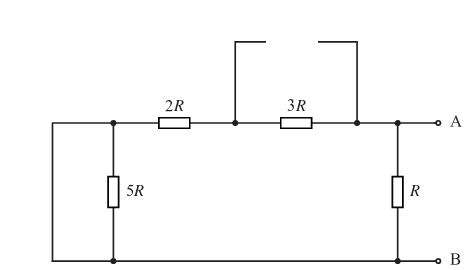
\includegraphics[scale=1.5]{katalog-1/ir-1.png} \\
\end{center}
Da der 5R Widerstand kurzgeschlossen ist, wird niemals Strom durch ihn hindurchfliessen. Somit können wir ihn durch einen Leerlauf ersetzen. \\
\begin{center}
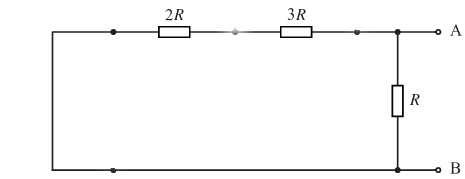
\includegraphics[scale=1.5]{katalog-1/ir-2.png} \\
\end{center}

2R und 3R liegen Seriell, somit können sie zu einem Widerstand der Grösse 5R zusammengefasst werden. \\
Dieser Widerstand ist wiederum parallel zu R, womit wir für den gesamten Widerstand und somit $R_E$ folgendes erhalten. \\
\begin{center}
  $R_E = (2R + 3R || R) = \frac{5R^2}{6R} = \frac{5}{6}R$
\end{center}

2) Nun müssen wir noch die Leerlaufspannung der Ersatzschaltung berechnen. Dazu wenden wir das Superpositionsprinzip an: \\
Zuerst berechnen wir die Spannung $U_{AB}$ zwischen den Klemmen A und B in Abhängigkeit der Spannungsquelle: \\


\begin{center}
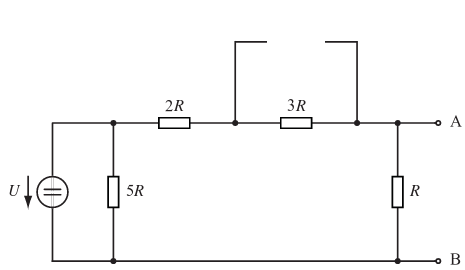
\includegraphics[scale=1.5]{katalog-1/uu-1.png}

\end{center}
\newpage
Die Widerstände 2R und 3R sind seriell.
\begin{center}
    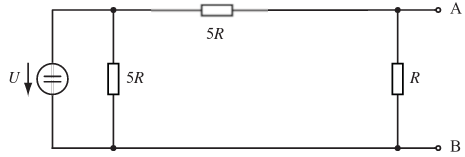
\includegraphics[scale=1.5]{katalog-1/uu-2.png}
\end{center}

Da die Widerstandände ($ 5R + R$ und $5R$) parallel sind, muss über beiden Ästen die Gleiche Spannung U abfallen. \\
Somit können wir die Spannungsteilerregel anwenden: \\
\begin{center}
    $U_{AB}^{(1)} = U \cdot \frac{R}{R + 5R} = U \cdot \frac{1}{6}$
\end{center}

Nun müssen wir noch die Spannung $U_{AB}^{(2)}$ in Abhängigkeit der Stromquelle berechnen: \\
Dazu setzen wir die Spannungsquelle zu 0:
\begin{center}
  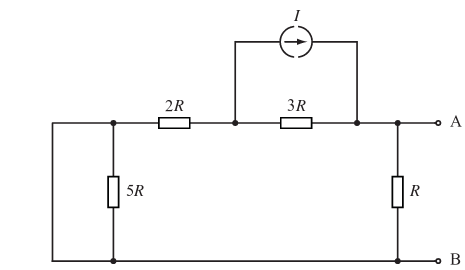
\includegraphics[scale=1.5]{katalog-1/iu-1.png}
\end{center}
Der Widerstand $R_5$ wird wieder kurzgeschlossen.
\begin{center}
  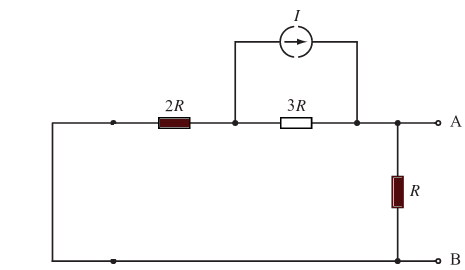
\includegraphics[scale=1.5]{katalog-1/iu-2.png}
\end{center}
Die Widerstäde $2R$ und $R$ können Seriell zusammengefasst werden, wodurch jedoch die Klemmen verschwinden :
\begin{center}
  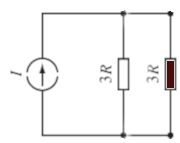
\includegraphics[scale=2.0]{katalog-1/iu-3.png} \\
\end{center}

Nun können wir mithilfe der Stromteilerregel den Strom durch den roten Widerstand berechnen:
\begin{center}
  $I_{Rot} = I \frac{3R}{3R + 3R} = \frac{I}{2}$
\end{center}

Dieser Strom fliesst durch die beiden Widerstände $R$ und $2R$ somit gilt für die Spannung über dem roten $R$ Widerstand und somit für die Spannung $U_{AB}^{(2)}$:
\begin{center}
  $U_{AB}^{(2)}  = U_R = I_{Rot}\cdot R = \frac{I\cdot R}{2}$
\end{center}

\newpage
Somit gilt für die Leerlaufspannung gemäss Superposition:
\begin{center}
  $U_{E} = U_{AB}^{(1)} + U_{AB}^{(2)} = \frac{U}{6} + \frac{I\cdot R}{2}$
\end{center}


b) Es gilt: $R_E = \frac{5}{6} \cdot 12 \Omega = 10\Omega$ und $U_E = 2V + 3A\cdot 6\Omega = 20V$ \\
Für $I_E$ gilt:
\begin{center}
  $I_E = \frac{U_E}{R_E} = \frac{20V}{10\Omega} = 2A$
\end{center}


c) Um die Leistung über dem Widerstand $R_2$ zu maximiere, schliessen wir zuerst das Lastnetzwerk an unsere Ersatzquelle an und ersetzen danach den Widerstand $R_2$ mit offenen Klemmen und Formen erneut das Netzwerk zu einer realen Quelle um. Aus der Vorlesung ist bekannt, dass die Leistung über $R_2$ genau dann maximal ist, wenn $R_2 = R_i$ gilt, wobei $R_i$ den Innenwiderstand gegenüber den Klemmen bezeichnet. \\
Die Aufgabe reduziert sich als darauf, den Innenwiderstand gegenüber den Klemmen zu berechnen.
\begin{center}
    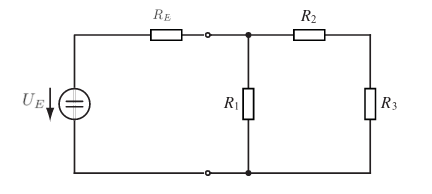
\includegraphics[scale=2.0]{katalog-1/lr-1.png}
        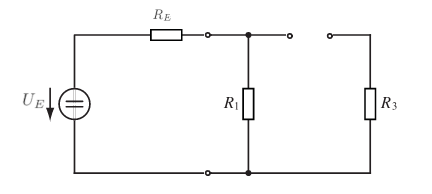
\includegraphics[scale=2.0]{katalog-1/lr-2.png}
\end{center}

Um den Innenwiderstand zu berechnen setzen wir die Quellen zu 0 und formen das Netzwerk um, bis nur noch ein Widerstand vorhanden ist. \\
\begin{center}

      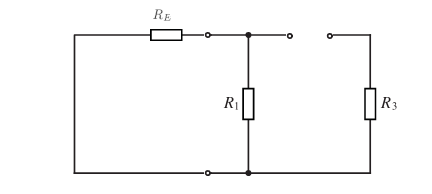
\includegraphics[scale=2.0]{katalog-1/lr-3.png}
\end{center}
Im ESB sind die Widerstände $R_E$ und $R_1$ parallel. Beide zusammen sind wiederum seriell zu $R_3$. Somit gilt für den Innenwiderstand: \\
$R_i = (R_E || R_1) + R_3$ \\
Um maximale Leistung an $R_2$ abzugeben, muss folgendes gelten:
\begin{center}
  $R_2 = R_i = (R_E || R_1) + R_3 \Rightarrow R_3 = R_2 - (R_E || R_1)$ \\
  $R_3 = 11.5 \Omega - (5\Omega || 20 \Omega) = 7.5 \Omega$
\end{center}

\newpage
d) Um den Spannungsabfall über $R_2$ zu berechnen, berechnen wir die Leerlaufspannung an den Klemmen:
\begin{center}
        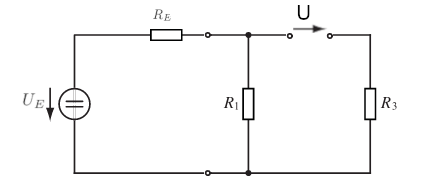
\includegraphics[scale=2.0]{katalog-1/lr-4.png} \\
\end{center}

Da durch den Widerstand $R_3$ kein Strom fliesst, gilt für die Spannung $U$:
\begin{center}
  $ U = U_{R_1} - U_{R_3} = U_{R_1} - 0A \cdot R_3 = U_{R_1}$
\end{center}
Die Spannung über $R_1$ können wir mithilfe des Spannungsteilers berechnen: \\
\begin{center}
  $U_{R_1} = U_E \cdot \frac{R_1}{R_E + R_1} = 15V \cdot \frac{20\Omega}{25\Omega} = 12V$
\end{center}
Aus der Vorlesung ist bekannt, dass bei maximaler Leistungabgabe, die Spannung über dem Lastwiderstand gerade die hälfte der Leerlaufspannung beträgt. Somit gilt für die Spannung über $R_2$:
\begin{center}
  $U_2 = \frac{U}{2} = 6V $ \\
  $P_2 = \frac{U_2^2}{R_2} = \frac{36V^2}{11.5\Omega} = 3.13W$
\end{center}

\end{homeworkProblem}




%----------------------------------------------------------------------------------------

\end{document}
